\appendix
\chapter{Verblisten für Operationalisierte Lernziele}\label{A_Verbliste}
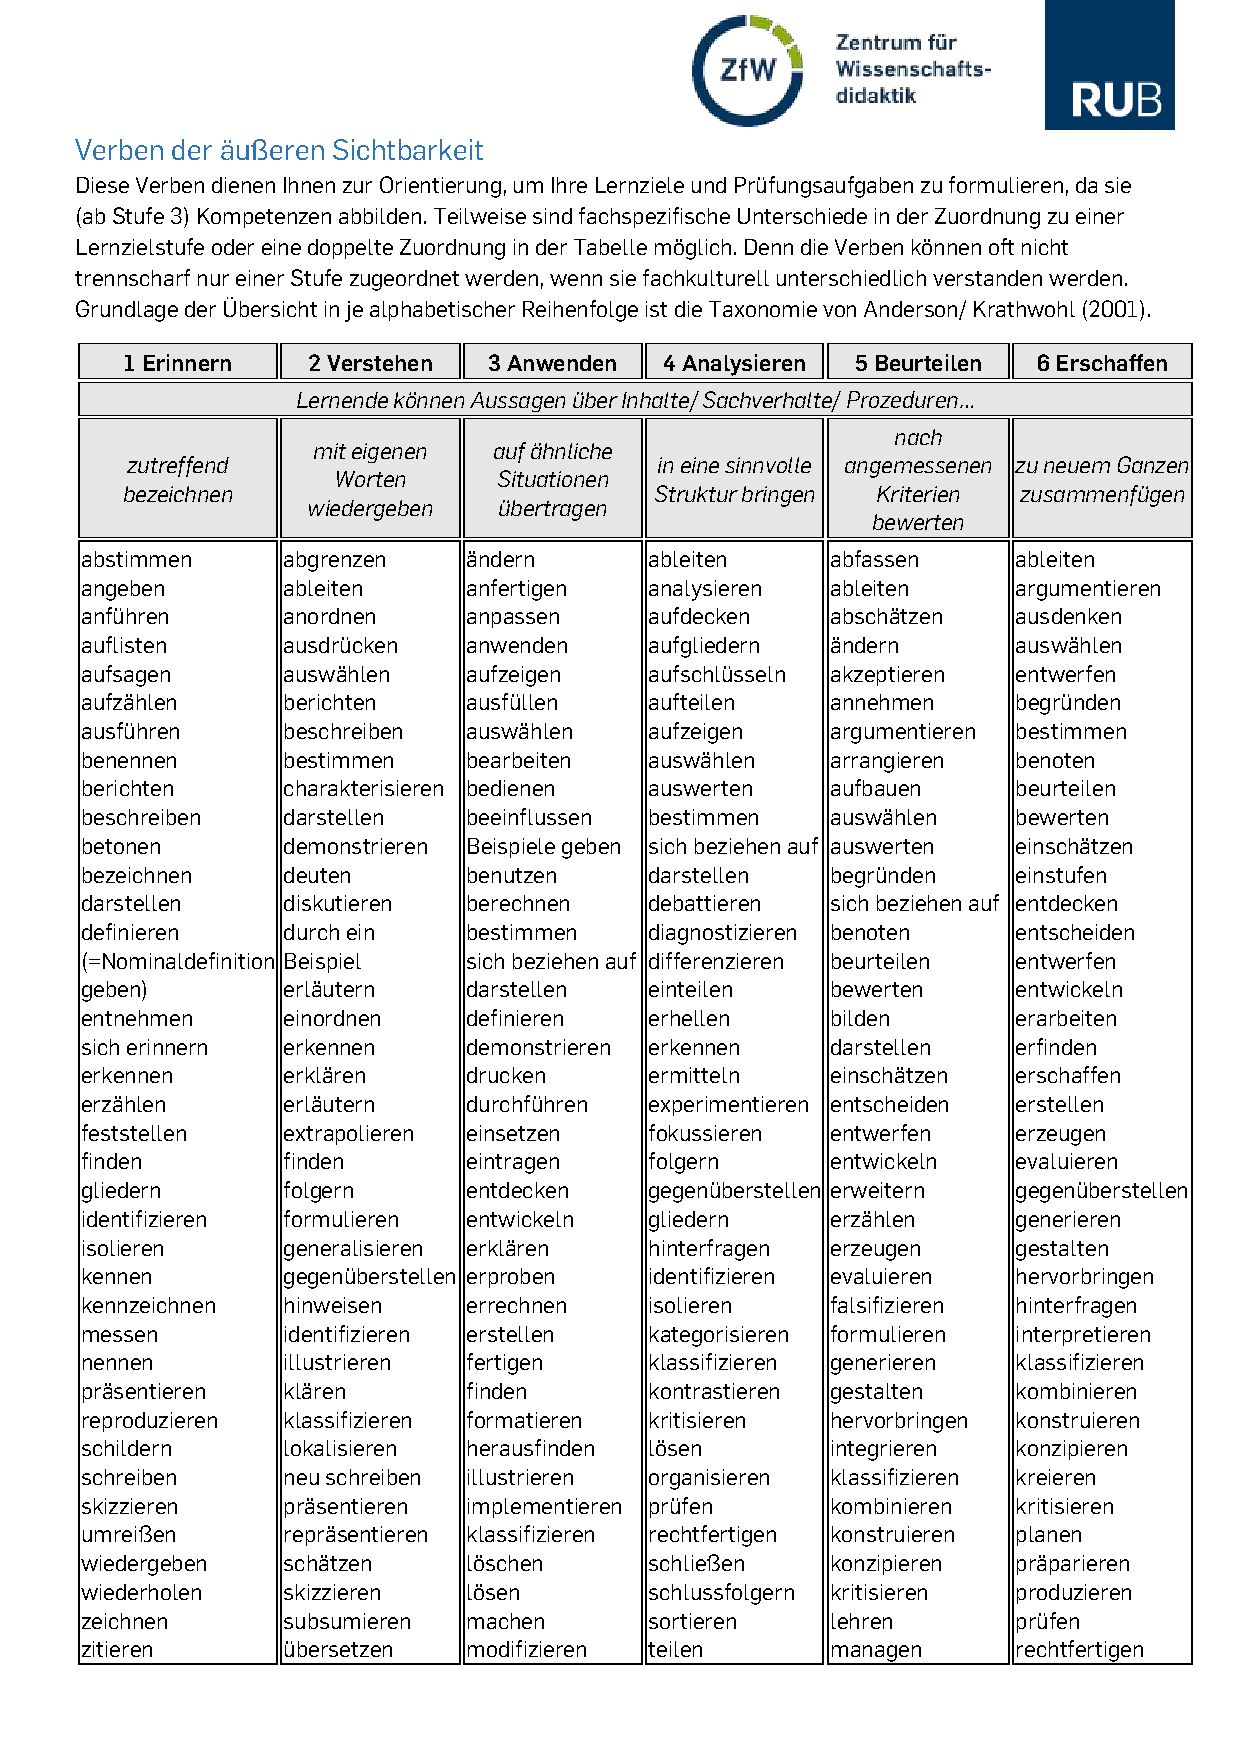
\includepdf[pages={1-2}]{Bilder/Verblisten_Kompetenz}

\chapter{Berliner Modell}\label{A_BerlinerModell}

\chapter{Weitere Artikulationsschemata}

\section{Grob-Phasen gem\"{a}{\ss} \textcite{DuitHausslerKircher}}
\begin{enumerate}
	\item {\bf Motivation} oder Einstiege
	\item {\bf Erarbeitung} Probleml\"{o}sung (beispielsweise im Experiment)
	\begin{enumerate}
	\item
	Planung des Experiments
	\item
	Durchf\"{u}hrung des Experiments
	\item
	Auswertung des Experiments
	\item
	R\"{u}ckblickende Er\"{o}rterung des Experiments
	\item
	Allgemeine Er\"{o}rterung
	\end{enumerate}
	\item {\bf Vertiefung} Integration, Behalten, Transfer.
\end{enumerate}

\section{\textcite{Ploeger}: Forschender Physikunterricht}
Konkret, anwendungsnah und auf den Punkt gebracht wird dieses Konzept in
\textcite{Ploeger} beschrieben.
Es finden sich dort auch viele Beispiele.
\begin{enumerate}
	\item {\bf Problemfrage}
	\item {\bf Vermutung}
	\item {\bf Versuchsplanung}
	\item {\bf Experiment}
	\item {\bf Auswertung}
\end{enumerate}
Der zentrale Unterschied zu Mothes ist die Sichtweise, aus der sie ihre Schemata formulieren. Während Mothes eher lehrerzentriert argumentiert, betont Plöger die aktive Beteiligung der Schüler an der Erarbeitung des Wissens.

\section{H.F.\ Bauer: Experimentalunterricht (1984)}
Das Grundschema des entdeckenden Unterrichts wird
hier spezialisiert-differenziert im Hinblick auf
das Experimentieren umgesetzt.

\mip Ziel des Unterrichts ist nicht Forschung an sich, sondern eine
Vertrautheit mit dem Forschen an sich.
	\begin{enumerate}
	\item {\bf Motivation}
	\item {\bf Problemherstellung}
	\item {\bf Meinungsbildung}
	\item {\bf Planen} und Konstruieren
	\item {\bf Laborieren --- Experimentieren}
	\item {\bf Schlie{\ss}en}
	\item {\bf Abstrahieren}
	\item {\bf Wissenssicherung durch Anwendung und \"{U}bung}
\end{enumerate}


\chapter{Beispiel einer didaktischen Analyse}\label{A_DidAna}